A central theme in the study of quantum magnetism has been the discovery and classification of materials hosting different types of collective excitations. This has unearthed a rich variety of ground state phases which can serve as non-trivial vacua, for example, for chiral topological excitations. Such excitations are promising for spintronics applications~\cite{wang_topological_2018} and are realized in a variety of magnetic phases: First,  topological magnon insulators (TMIs) are conventional long-range spin ordered magnets whose bulk magnon bands have nonzero topological invariants. As a result they can display magnon surface states with uni-directional propagation~\cite{katsura_theory_2010,zhang_topological_2013,mook_edge_2014,mcclarty_topological_2022}. A second example beyond conventional ordered magnets are  valence bond solids (VBS), which have a gapped dimer singlet ground state, and may host chiral boundary modes of triplon excitations. These were first predicted for the Shastry-Sutherland model system SrCu$_2$(BO$_3$)$_2$, where the addition of Dzyaloshinskii-Moriya (DM) interactions leads to a spin-orbit type coupling of triplons, such that gaps induced by a small magnetic field endow the triplon bands with a non-zero Chern number~\cite{romhanyi_hall_2015, mcclarty_topological_2017,malki_magnetic_2017}.   
The third and most exotic example are quantum spin liquids (QSLs) with topologically ordered ground states~\cite{savary_quantum_2017,zhou_quantum_2017,knolle_field_2019}. Chiral QSLs with broken time reversal symmetry (TRS) can host fractionalized surface modes with unidirectional propagation akin to their electronic brethren of the (fractional) quantum Hall effect~\cite{kalmeyer_equivalence_1987}. 

Finding stable chiral excitations in microscopic models of insulating magnets has turned out to be a major challenge. Often, the ground states themselves are very fragile, as has been the case for many QSLs~\cite{szasz_chiral_2020,chen_quantum_2022}, or the topological edge excitations may be unstable to decay processes from interactions~\cite{chernyshev_damped_2016,habel_breakdown_2023}. In this context, the Kitaev honeycomb model with its bond-anisotropic Ising interactions stands out as a rigorous example of a stable QSL~\cite{kitaev_anyons_2006} and a robust TMI phase in large magnetic fields~\cite{mcclarty_topological_2018,joshi_topological_2017}. For small magnetic field the gapless Kitaev QSL turns into a gapped QSL with chiral Majorana boundary modes. Moreover, the presence of perturbing interactions like Heisenberg exchange present in any real materials' realization gives rise to a rich phase diagram with various long-range ordered magnetic phases~\cite{chaloupka_zigzag_2013,rau_spin-orbit_2016} and, surprisingly, TMI behavior in the field-polarized regime~\cite{mcclarty_topological_2018,joshi_topological_2017}. Hence, excitations of the (extended) Kitaev honeycomb model can be tuned from chiral Majorana excitations to stable chiral magnons as a function of increasing magnetic field. This is not only interesting theoretically but of direct experimental relevance because chiral magnetic excitations give rise to a thermal Hall response~\cite{katsura_theory_2010,matsumoto_theoretical_2011}. The latter has been measured in the Kitaev magnet $\alpha$-RuCl$_3$~\cite{kasahara_majorana_2018,bruin_majorana_2022}, but whether its origin is related to QSL or TMI behavior is still under debate~\cite{czajka_planar_2023,chern_sign_2021}.  

Following Kitaev's original proposal for the honeycomb lattice~\cite{kitaev_anyons_2006} subsequent work established that his model can be exactly solved on a wide variety of lattices with coordination number three, e.g.~different 2D and 3D lattices ~\cite{yao_exact_2007,mandal_exactly_2009,hermanns_quantum_2014,obrien_classification_2016,peri_non-abelian_2020} and even disordered amorphous lattices~\cite{grushin_amorphous_2023}. 
A particularly interesting case is the star lattice -- a honeycomb lattice with each vertex decorated by a triangle as shown in fig.~\ref{fig:star_lattice_and_jk}a -- where the Kitaev QSL was the first rigorous example of a chiral QSL breaking TRS {\it spontaneously}~\cite{yao_exact_2007}. The presence of plaquettes with an odd number of sites leads to broken TRS in a given flux configuration, such that the zero flux ground state is a chiral QSL with Majorana edge modes. Despite much research on the stability of the Kitaev QSL on the honeycomb lattice~\cite{winter_models_2017,hermanns_physics_2018,trebst_kitaev_2022} the effect of perturbing interactions on the chiral Kitaev QSL has not been investigated on the star lattice. This is even more surprising given that the pure antiferromagnetic Heisenberg model on the star lattice is one of the rare established examples hosting a singlet VBS ground state phase with triplon excitations~\cite{richter_absence_2004,choy_classification_2009,yang_competing_2010, jahromi_spin-frac12_2018,jahromi_infinite_2018,ran_emergent_2018}. Additional motivation comes from the recent synthesis of the first $S=1/2$ materials realisation of the star lattice~\cite{sorolla_synthesis_2020,ji_dielectric_2022} (previous star lattice realisations contained $S=5/2$ spin clusters~\cite{zheng_star_2007}).  


In this paper we investigate the rich ground state phase diagram and distinct types of chiral excitations of the  Kitaev-Heisenberg model on the star lattice. We show that, in addition to the chiral Kitaev QSL and various magnetically ordered phases, a novel bond-anisotropic triplet VBS is realized. The triplon bands show non-zero Chern numbers once a small magnetic field is included to induce gaps. Thus, we establish that -- in analogy to the honeycomb Kitaev model, which can be tuned with a magnetic field from hosting chiral Majorana to chiral magnon excitations -- the Kitaev-Heisenberg model on the star lattice tunes from chiral Majoranas to chiral triplons. 

One of the competing phases that can form in lieu of magnetic order or QSLs are VBSs. In their most common form, neighbouring pairs of spins anti-align into singlets, forming a dimer covering of the entire lattice. On this background, excitations involve breaking a singlet state and creating a spin-1 triplet -- a so-called triplon mode that can be represented as a bosonic particle~\cite{sachdev_bond-operator_1990}. Recently, interest has been generated in triplons as a way of realising a bosonic bulk-boundary correspondence. This has been proposed both in 1D topological chain systems~\cite{joshi_topological_2017}, as well as 2D bosonic analogues of the quantum Hall effect~\cite{romhanyi_effect_2011,romhanyi_hall_2015,mcclarty_topological_2017, nawa_triplon_2019, malki_magnetic_2017}. In general, such effects have relied on the presence of Dzyaloshinskii-Moriya (DM) interactions to generate complex hoppings in the triplon Hamiltonian, allowing for for non-zero Chern and winding numbers to appear. Here, we will show that the Kitaev interaction provides an alternative route for a triplon Hall state forming in the absence of DM interactions. For Heisenberg-Kitaev model on the star lattice we unearth an extremely rich phase diagram containing singlet and triplet VBSs with a wide range of Chern numbers.

The structure of this chapter is as follows. 
First we introduce the model, describing the parameters used to tune the system and discussing previous studies that have looked at both the star and the honeycomb lattices. Following this, our investigation is composed of three parts. 
In \textsection\ref{sec:triplons_dmrg} we start by numerically characterising the ground state phase diagram using infinite density matrix renormalisation group (iDMRG) methods. In particular, we find two phases in the star lattice that do not have an analogue on the Honeycomb lattice, where geometric frustration leads to the formation of a VBS ground state. We will also present a \textit{four-unit-cell spin rotation} that reveals a hidden isometry of the ground state phase diagram. We show that the four non-spin liquid phases may be categorised into two sets, which are equivalent under this transformation.
In \textsection\ref{sec:majorana_mft} we construct a parton Majorana mean field description that corroborates the ground state phase diagram, and allows us to determine the topological properties of the bands and the presence of chiral Majorana excitations in the extended KSL regime. 
Finally, in \textsection\ref{sec:triplon_bond_operator} we  construct a bosonic mean field theory describing the triplon excitations of the VBS phase. The topological properties of the triplon phases are derived and we confirm the existence of topologically protected triplon edge modes. 
\begin{figure}[t]
    \centering
    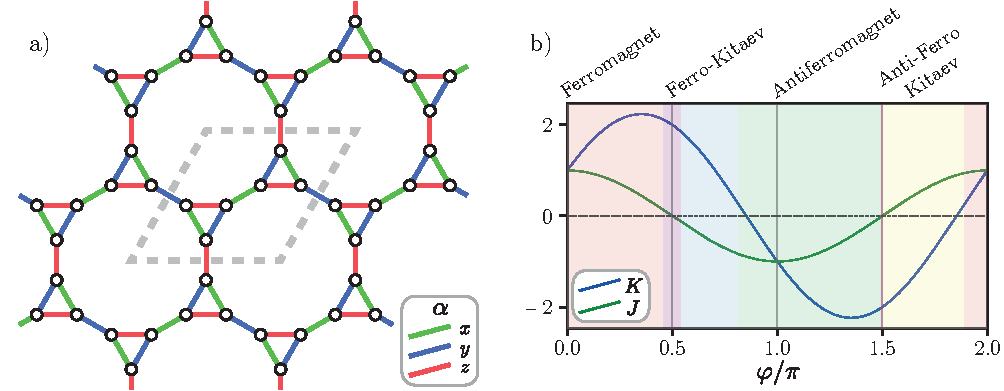
\includegraphics[]{kitaev_heisenberg_star/figures/star_lattice.pdf}
    \caption{ 
        \textbf{(a)} A fragment of the star lattice is shown. Bond labelling is indicated by the colouring, and the six-site unit cell is depicted with a grey dashed rhombus.
        \textbf{(b)} The dependence of the $J$ and $K$ values on the parameter $\varphi$ is shown. The two pure Heisenberg and two pure Kitaev points are labelled. The background colouring corresponds to the phase boundaries obtained in \textsection\ref{sec:triplons_dmrg}.
    }
    \label{fig:star_lattice_and_jk}
\end{figure}

Let us start by defining the model, which we shall construct on the star lattice shown in fig.~\ref{fig:star_lattice_and_jk}a. As in the previous chapter, each site hosts a single spin-1/2, and bonds are coloured with a label $\alpha \in \{x,y,z\}$ such that no vertex touches two bonds of the same colour. We choose the Hamiltonian to interpolate between two well-studied limits: the spin isotropic Heisenberg and the anisotropic Kitaev limit. In the Heisenberg limit, adjacent spins are coupled with an isotropic $\mathbf{\sigma}_j \cdot \mathbf{\sigma}_k$ coupling. In the Kitaev limit each bond of type $\alpha$ is coupled by a $\sigma_j^\alpha \sigma_k^\alpha$, thus only in the direction that matches the colouring.
\begin{align} \label{eqn:kitave_heisenberg_hamiltonian}
    H = -
    \sum_{\braket{jk}_\alpha } \bigg (K \sigma_j^\alpha \sigma_k^\alpha
    +J \sum_{\bar \alpha \neq \alpha}  \sigma_j^{\bar \alpha} \sigma_k^{\bar \alpha}
    \bigg ).
\end{align}
Here $\braket{jk}_\alpha$ indicates a bond of type $\alpha$ that connects adjacent sites $j$ and $k$. The parameter $K$ determines the strength of the ``on-colouring'' coupling, where the coupling direction matches $\alpha$, and $J$ determines the strength of the two remaining ``off-colouring'' couplings. In analogy with previous studies~\cite{chaloupka_zigzag_2013, gohlke_dynamics_2017}, let us introduce a single parameter $\varphi \in [0,2\pi]$ that smoothly maps onto the possibilities for $K$ and $J$ according to
\begin{align} \begin{aligned} \label{eqn:phi_def}
    K &= 2\sin \varphi + \cos \varphi, \\
    J &= \cos \varphi,
\end{aligned}\end{align}
shown in fig.~\ref{fig:star_lattice_and_jk}b. 